% Full instructions available at:
% https://github.com/elauksap/focus-beamertheme

\documentclass{beamer}
\usetheme{focus}

\title{CoPL \\ Object Oriented Programming}
\subtitle{Crashcourse}
\author{Daan Wichmann}
% \titlegraphic{\includegraphics[scale=1.25]{focuslogo.pdf}}
\institute{Radboud University}
\date{10 03 2026}

\usepackage{minted}
\usepackage{emoji}

\begin{document}
    \begin{frame}
        \maketitle 
    \end{frame}

    \begin{frame}{Before we start}
        \begin{itemize}
            \item Lot's of topics to cover, limited time per topic
            \item Assuming basic Python knowledge from Programming 1 \& Programming 2.
        \end{itemize}
    \end{frame}
    
    \section{Objects \& Methods}
\begin{frame}{What are objects?}
    \pause
    \begin{block}{Objects}
        \textbf{Objects} are Python's abstraction for data. All data in a Python program is represented by objects or by relations between objects.
    \end{block}
\end{frame}

\begin{frame}{What are objects?}
\pause
    The following are objects in Python:
    \begin{itemize}
        \pause
        \item Integers (e.g. 127) \pause
        \item Strings (e.g. "CognAC")\pause
        \item Lists (e.g. ["Damai", "Daan", "Ella"])\pause
        \item \textbf{Every value in Python!}
    \end{itemize}
\end{frame}

\begin{frame}{What are methods?}
    \pause
    \begin{block}{Methods}
        \textbf{Methods} are functions that belong to a certain \textbf{type of object}.
    \end{block}
    \begin{itemize}
        \pause
        \item You call methods on an object.
        \pause
        \item Methods that belong to a certain type of object, can not be called on another type of object
    \end{itemize}
\end{frame}

\begin{frame}[fragile]{What are methods?}
You have already seen a lot of methods!
\pause
\begin{minted}{python}
my_list = [1, 2, 3]
\end{minted} 
\pause
\begin{minted}{python}
my_list.append(4)
\end{minted}
\pause
\begin{minted}{python}
print(my_list)
>>> [1, 2, 3, 4]
\end{minted} 
\pause
\textbf{append} is a \textbf{method} of {lists}.
\end{frame}

\begin{frame}[fragile]{What are methods? Another example.}
\pause
\begin{minted}{python}
my_string = "daan"  # Note: all lowercase
\end{minted} 
\pause
\begin{minted}{python}
my_capitalized_string = my_string.capitalize()
\end{minted}
\pause
\begin{minted}{python}
print(my_capitalized_string)
>>> "Daan"
\end{minted} 
\pause
\textbf{capitalize} is a \textbf{method} of {strings}.
\end{frame}

\begin{frame}[fragile]{What are methods?}
\pause
\begin{minted}{python}
my_list = [1, 2, 3]
\end{minted} 
\pause
\begin{minted}{python}[breaklines]
my_list.capitalize()
\end{minted}
\pause
\begin{minted}{python}
>>> AttributeError
\end{minted} 
\pause
\textbf{Why?}
\textit{'capitalize' is not a method of 'list'}
\end{frame}



    \section{Classes}

\begin{frame}{What are classes?}
\pause
\begin{block}{Class (definition)}
    A class is a blueprint for a type of object, defining it's \textbf{data attributes} and \textbf{methods}.
\end{block}
\pause
\begin{alertblock}{Terminology}
    We call an object from a certain class, an \textbf{instance} of that class. E.g. "OOP" is an instance of the class str (string).
\end{alertblock}
\end{frame}

\begin{frame}{Why do we use classes?}
    \pause
    \begin{itemize}
        \pause
        \item Python only gives us a limited amount of types, integers, floats, strings, etcetera. 
        \pause
        \item With classes we can extend this and model anything we want!
        \pause
        \begin{itemize}
            \item Like students, bank accounts, courses, shopping cart.
        \end{itemize}
        \pause
        \item Encapsulation (later)
        \pause
        \item Seperation of Concerns (later)
    \end{itemize}
\end{frame}

\begin{frame}{What do classes consist of?}
    \begin{itemize}
        \pause
        \item Methods (behaviour)
        \pause
        \item Data Attributes (properties/fields)
    \end{itemize}
\end{frame}

\begin{frame}{What do classes consist of?}
    \pause
    Data Attributes:
    \begin{itemize}
        \pause
        \item Variables that belong to a single object
        \pause
        \item For example a person can have the following data variables (i.e. data attributes) which we would like to store:
        \pause
        \begin{itemize}
            \item first name (string)
            \item last name (string)
            \item age (int)
        \end{itemize}
        \pause
        \item These variables can be of any type! (Strings, integers, lists, and also objects of other classes)
    \end{itemize}
\end{frame}

\begin{frame}{Methods}
\begin{itemize}
    \item You have already seen a lot of methods
    \pause
    \item For example, for a person we could have:
    \begin{itemize}
        \pause
        \item Speak
        \item Dance
        \item Study
    \end{itemize}
    \pause
    \item Every class needs one special method:
    \begin{itemize}
        \pause
        \item \textbf{The constructor}
    \end{itemize}
\end{itemize}
\end{frame}

\begin{frame}{What is a constructor?}
\pause
\begin{block}{Constructor}
In Python, a \textbf{constructor} is a special method called when an object is created. It initializes all data attributes.
\end{block}
\end{frame}

\begin{frame}[fragile]{The constructor}
To create objects of a certain class:
\pause
\begin{minted}{python}
my_string = "CognAC"  # Class str
my_int = 18  # Class int
my_list = [18, 2003]  # Class list
\end{minted}
\pause
\textbf{But what if we have a new type of object of a new class, for example a Fraction class}
\pause
\textit{We use the constructor!}
\end{frame}

\begin{frame}[fragile]{The constructor}
\begin{minted}{python}
# We import the class from the module 'fractions'
# Classes always start with a capital lette
from fractions import Fraction
\end{minted}{python}
\pause
\begin{minted}{python}
# We call the constructor by 'calling the class',
# this creates a new object for us!
# The constructor takes two arguments:
# numerator and denominator (in this case 8 and 10)
my_fraction = Fraction(8, 10)  # Fraction of 8/10th
\end{minted}
\end{frame}

\begin{frame}{Making our own class!}
\begin{itemize}
    \pause
    \item We now have all ingredients to create our own classes!
    \pause
    \item Let's say we want to model a person in python
    \pause
    \item We want it to have a \textit{first name, last name, age} (data attributes)
    \pause
    \item And we want a person to 'speak' i.e. print some text (methods)
    \pause
    \item We create our own class \textbf{Person}
\end{itemize}
\end{frame}

\begin{frame}[fragile]{Creating our Person class}
\begin{minted}[fontsize=\footnotesize, breaklines]{python}
class Person():
\end{minted}
\pause
\begin{minted}[fontsize=\footnotesize, breaklines]{python}
    
    # The constructor
    def __init__(self, first_name, last_name, age):
        self.first_name = first_name  # Data attribute
        self.last_name = last_name  # Data attribute
        self.age = age  # Data attribute
\end{minted}
\pause
\begin{minted}[fontsize=\footnotesize, breaklines]{python}

    # Method
    def speak(self):
        print(f"Hey, my name is {self.first_name}")
\end{minted}
\end{frame}

\begin{frame}{The 'self' parameter}
\begin{itemize}
    \pause
    \item The first parameter in a constructor definition is always named \textbf{self}. 
    \pause
    \item This refers to the object itself, and is necessary for declaring any data attributes attached to the object.
    \pause
    \item It is automatically filled in by the interpreter with the object it is called on.
\end{itemize}
\end{frame}

\begin{frame}[fragile]{Creating our Person class}
\begin{minted}[fontsize=\footnotesize, breaklines]{python}
class Person():
    
    # The constructor
    def __init__(self, first_name, last_name, age):
        self.first_name = first_name  # Data attribute
        self.last_name = last_name  # Data attribute
        self.age = age  # Data attribute

    # Method
    def speak(self):
        print(f"Hey, my name is {self.first_name}")
\end{minted}
\end{frame}

\begin{frame}[fragile]{Data Attributes}
Accessing a data attribute:
\pause
\begin{minted}{python}
person = Person("Daan", "Wichmann", "Secret")
\end{minted}
\pause
\begin{minted}{python}
print(person.first_name)
>>> "Daan"
\end{minted}
\end{frame}

\begin{frame}[fragile]{Data Attributes}
Re-assigning an attribute:
\pause
\begin{minted}{python}
person = Person("Daan", "Wichmann", "Secret")
\end{minted}
\pause
\begin{minted}{python}
person.first_name = "Damai"
print(person.first_name)
>>> "Damai"
\end{minted}
\end{frame}

\begin{frame}[fragile]{Our beautiful class}
\begin{minted}{python}
class Person():
    
    # The constructor
    def __init__(self, first_name, last_name, age):
        self.first_name = first_name  # Attribute
        self.last_name = last_name  # Attribute
        self.age = age  # Attribute

    # Method
    def speak(self):
        print(f"Hey, my name is {self.first_name}")
\end{minted}
\end{frame}

\begin{frame}[fragile]{Calling our method}
\pause
\begin{minted}{python}
person = Person("Daan", "Wichmann", "Secret")
\end{minted}
\pause
\begin{minted}{python}
person.speak()
>>> Hey, my name is Daan
# Note that we don't fulfill the 'self' 
# parameter, but the interpreter
# does it automatically for us.
\end{minted}
\end{frame}

\begin{frame}{Why?}
Why do we want to use classes?
\begin{itemize}
    \item If we want to to represent something that is not already in Python
    \item To make collaboration easier
    \item If we want to 'group together' functionality
\end{itemize}
\end{frame}


    \section{Objects \& References}

\begin{frame}[plain]
What do our variables store exactly?
\end{frame}

\begin{frame}[fragile]{References}
\begin{minted}{python}
person1 = Person("Daan", "Wichmann", "Secret")
\end{minted} 

\pause
\begin{minted}{python}[breaklines]
person2 = person1
\end{minted}

\pause
\begin{minted}{python}
person3 = Person("Damai", "Jiworo", "Secret")
\end{minted} 
\end{frame}

\setbeamertemplate{caption}[numbered]
\begin{frame}{Memory model}
    \begin{figure}
        \centering
        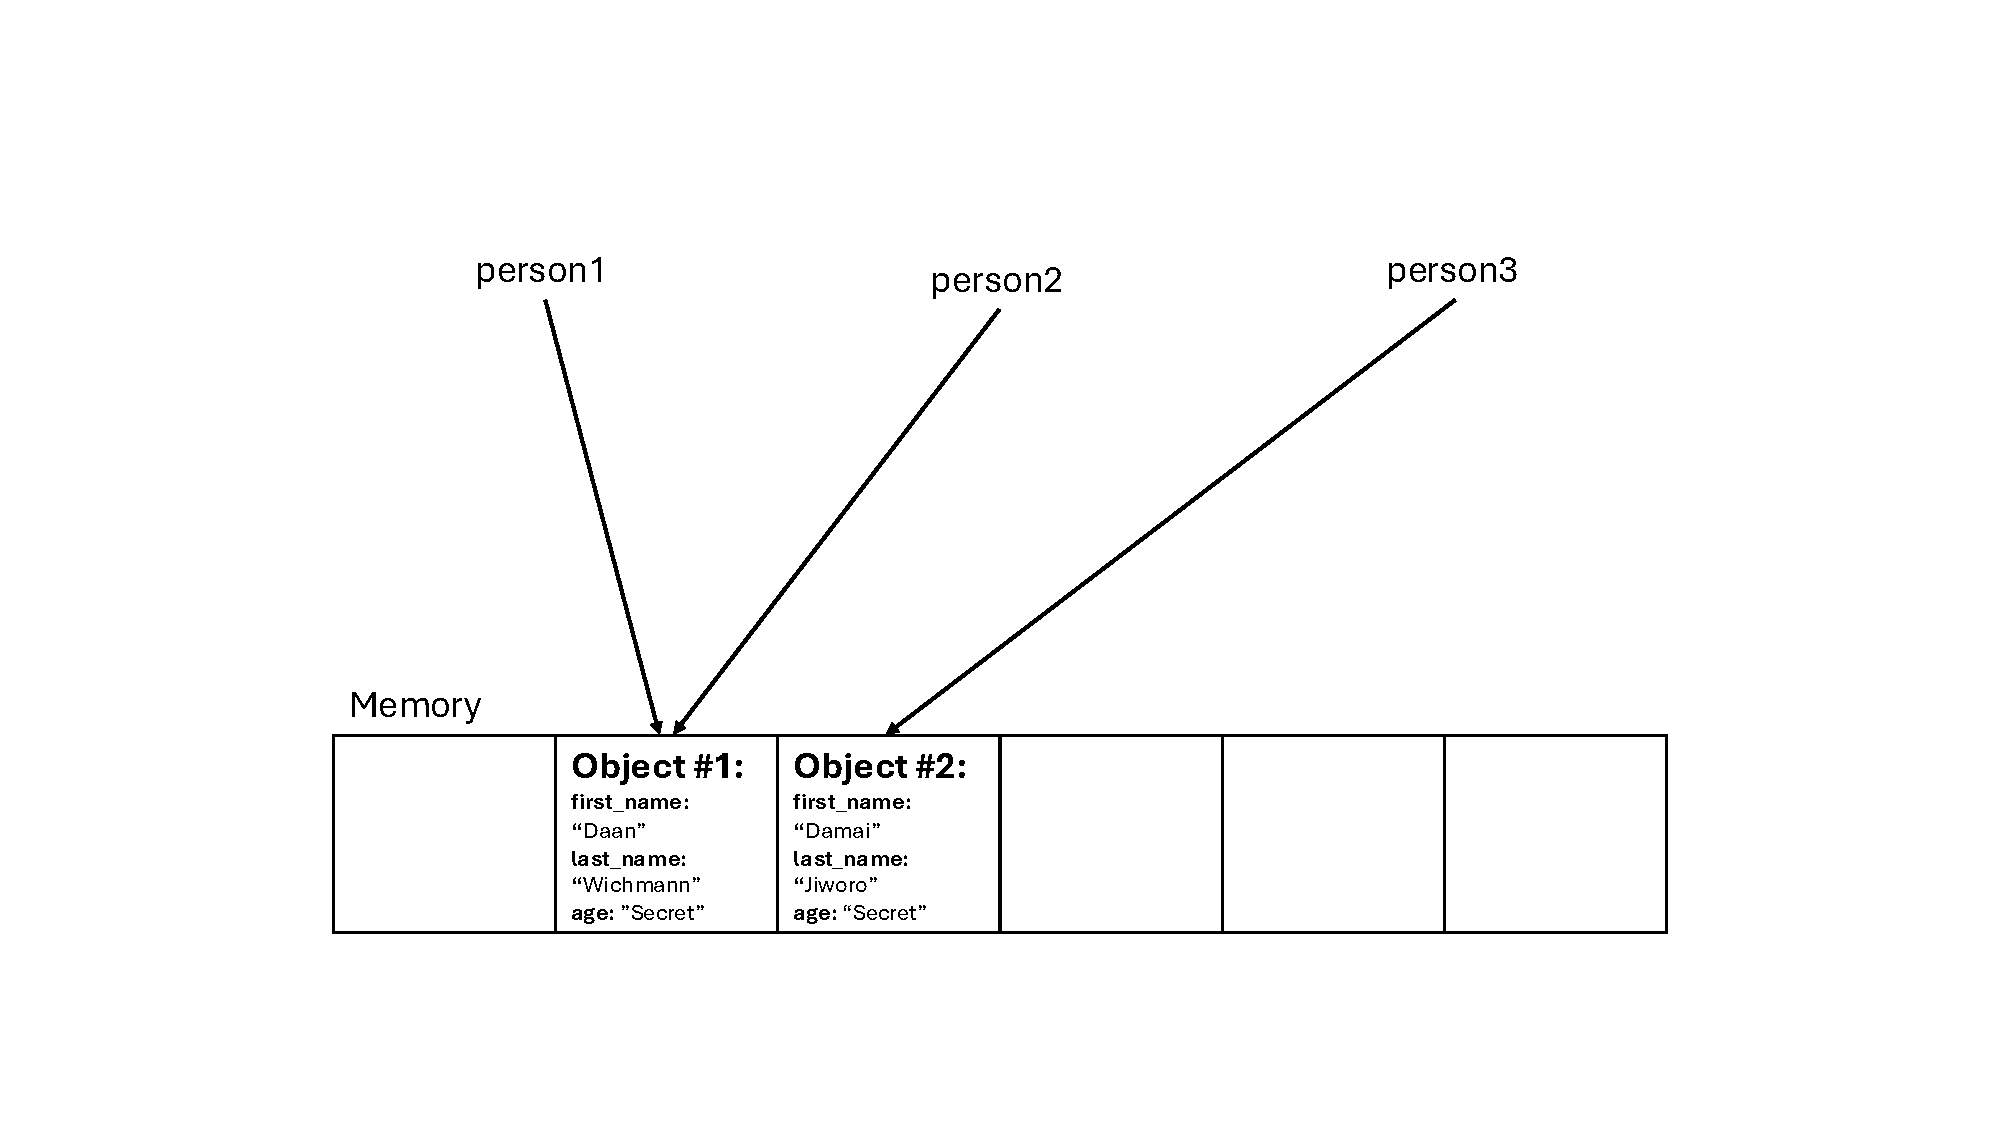
\includegraphics[scale=0.30]{images/memory.pdf}
        \caption{Simplified memory model}
        \label{fig:focuslogo}
    \end{figure}
\end{frame}

\begin{frame}[fragile]{Small quiz}
\begin{minted}{python}
person1 = Person("Damai", "Jiworo", "Secret")
\end{minted}
\pause
\begin{minted}{python}
person2 = person1
\end{minted}
\pause
\begin{minted}{python}
person3 = Person("Daan", "Wichmann", "Secret")
\end{minted} 
\pause
\begin{minted}{python}
person2.first_name = "Emma"
\end{minted}
\pause
\begin{minted}{python}
print(person1.first_name)  # What is the output?
\end{minted}
\pause
\begin{minted}{python}
>>> "Emma"
\end{minted}
\end{frame}

\begin{frame}[fragile]{Another one}
\begin{minted}{python}
person1 = Person("Damai", "Jiworo", "Secret")
\end{minted}
\pause
\begin{minted}{python}
person2 = Person("Damai", "Jiworo", "Secret")
\end{minted} 
\pause
\begin{minted}{python}
person2.first_name = "Emma"
\end{minted}
\pause
\begin{minted}{python}
print(person1.first_name)  # What is the output?
\end{minted}
\pause
\begin{minted}{python}
>>> "Damai"
\end{minted}
\end{frame}

    \begin{frame}[plain]
        Part 1 of 3 done! Break?
    \end{frame}

    \section{Inheritance}

\begin{frame}{New idea... new problem...}
    \begin{itemize}
        \pause
        \item We have now modeled a person with our \textit{Person} class
        \pause
        \item What if we want to model a student?
        \pause
        \item A student is also a person!
        \begin{itemize}
            \pause
            \item \textbf{Duplicate code}
        \end{itemize}
        \pause
        \item What is the best way to model this?
        \begin{itemize}
            \pause
            \item using \textbf{Inheritance!}
        \end{itemize}
    \end{itemize}
\end{frame}

\begin{frame}[plain]
So, what is inheritance?
\end{frame}

\begin{frame}{Inheritance}
    Lets look at the definition in the context of biology
    \pause
    \begin{block}{Inheritance (Biology)}
    Inheritance is the way that genetic information is passed from a parent to a child. Members of the same biological family tend to have similar characteristics
    \end{block}
\end{frame}

\begin{frame}{Inheritance}
    Lets translate this to OOP!
    \pause
    \begin{block}{Inheritance (OOP)}
    Inheritance is the concept in which a class can \textit{inherit} \textbf{data attributes} and \textbf{methods} from another class. Here, the class that inherits, is called the \textbf{derived class}. The class that the derived class inherits from, is called the \textbf{base class}.
    \end{block}
    \pause
    \begin{alertblock}{Alternative terminology}
        Inheriting is sometimes called \textbf{deriving}. So you can also say, the derived class \textbf{derives} data attributes and methods from it's base class.
    \end{alertblock}
\end{frame}

\begin{frame}{Inheritance}
    In the case of our example:
    \begin{block}{Inheritance (OOP)}
    Inheritance is the concept in which a class (\textbf{Student}) can \textit{inherit} data attributes (\textbf{first\_name, last\_name, age}) and methods (\textbf{speak()}) from another class (\textbf{Person}). The class that the derived class inherits from, is called the \textbf{base class}.
    \end{block}
    \begin{alertblock}{Alternative terminology}
        Inheriting is sometimes called \textbf{deriving}. So you can also say, the derived class \textbf{derives} data attributes and methods from it's base class.
    \end{alertblock}
\end{frame}

\begin{frame}{What can we do with inheritance?}
\begin{itemize}
    \item Create a \textbf{hierarchy} of classes (i.e. a class hierarchy :D) which describes their relationship (e.g. a Student is a Person, but not the other way around)
    \item Avoid writing duplicate code!
    \item \textbf{Encapsulation} (more on that later)
\end{itemize}    
\end{frame}

\begin{frame}[plain]
Let's look at the class hierarchy of our example!
\end{frame}

\begin{frame}{Hierarchies}
    \begin{figure}
        \centering
        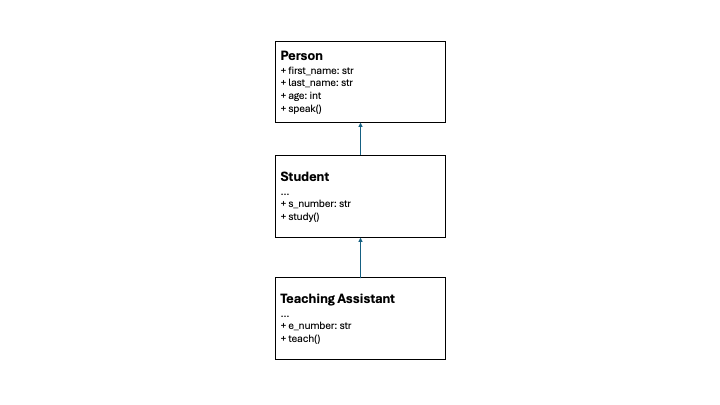
\includegraphics[scale=0.30]{images/hierarchy.png}
        \caption{our hierarchy}
        \label{fig:focuslogo}
    \end{figure}
    \pause
    \textbf{Note:} Inheriting classes (Student) can also be inherited from (TeachingAssistant)!
\end{frame}

\begin{frame}[plain]
Surprise quiz (no grade)
\end{frame}

\begin{frame}{Inheritance quiz}
What is the \textit{base class} of \textit{Student}?
\pause
\begin{itemize}
    \item \textbf{Answer:} Person
\end{itemize}
\pause
\person
Which class is \textit{Student} a \textit{derived class} of?
\pause
\begin{itemize}
    \item \textbf{Answer:} Person
\end{itemize}
\pause
What is a \textit{derived class} of \textit{Student}?
\pause
\begin{itemize}
    \item \textbf{Answer:} TeachingAssistant
\end{itemize}
\pause
Which data attributes does \textit{TeachingAssistant} inherit?
\pause
\begin{itemize}
    \item \textbf{Answer:} first\_name, last\_name, age, and s\_number
\end{itemize}
\pause
Which class is \textit{TeachingAssistant} a \textit{derived class} of?
\pause
\begin{itemize}
    \item \textbf{Answer:} Person and Student (sorry, it's both)
\end{itemize}
\end{frame}

\begin{frame}[plain]
How do we implement this in Python?
\end{frame}

\begin{frame}[fragile]{Remember our beautiful class}
\begin{minted}{python}
class Person():
    
    # The constructor
    def __init__(self, first_name, last_name, age):
        self.first_name = first_name  # Attribute
        self.last_name = last_name  # Attribute
        self.age = age  # Attribute

    # Method
    def speak(self):
        print(f"Hey, my name is {self.first_name}")
\end{minted}
\end{frame}

\begin{frame}[fragile]{Let's derive from it}
\begin{minted}[fontsize=\footnotesize]{python}
class Student(Person):

\end{minted}
\pause
\begin{minted}[fontsize=\footnotesize]{Python}
    # The constructor
    def __init__(self, first_name, last_name, age, s_number):
    
        # Calling the constructor of base class
        super().__init__(first_name, last_name, age)
        self.s_number = s_number

    # Method
    def study(self):
        print(f"Student {self.s_number} is studying!")
\end{minted}
\end{frame}

\begin{frame}{The super() function}
\begin{block}{super()}
The \textbf{super()} function refers to the base class of the class. We can use it to access/call methods of the base class.
\end{block}
If we call a method on the super() function, it is just like we would call it on \textbf{self}, but than as if it were an object of the base class!
\end{frame}

\begin{frame}[fragile]{Lets test it}
\pause
\begin{minted}[fontsize=\footnotesize]{python}
student = Student("Daan", "Wichmann", "secret", "secret")
\end{minted}
\pause
\begin{minted}[fontsize=\footnotesize]{python}
student.speak()
>>> Hey, my name is Daan
\end{minted}
\pause
\begin{minted}[fontsize=\footnotesize]{python}
student.study()
>>> Student secret is studying!
\end{minted}
\end{frame}

\begin{frame}{Hierarchies - Another example}
    \begin{figure}
        \centering
        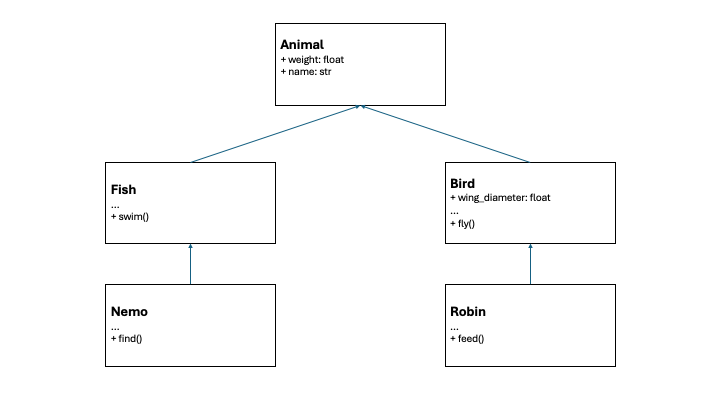
\includegraphics[scale=0.30]{images/hierarchy_another_example.png}
        \caption{Another example}
        \label{fig:focuslogo}
    \end{figure}
\end{frame}


    \section{Method overriding}

\begin{frame}{Overriding}
\begin{itemize}
    \item What if we want Student's \textit{speak()} to do something different from Person's \textit{speak()}?
    \item We can \textbf{override} the method! (\textbf{Method overriding})
\end{itemize}
\end{frame}

\begin{frame}[fragile]{Our beautiful class again}
\begin{minted}{python}
class Person():
    
    # The constructor
    def __init__(self, first_name, last_name, age):
        self.first_name = first_name  # Attribute
        self.last_name = last_name  # Attribute
        self.age = age  # Attribute

    # Method
    def speak(self):
        print(f"Hey, my name is {self.first_name}")
\end{minted}
\end{frame}

\begin{frame}[fragile]{And its subclass}
\begin{minted}[fontsize=\footnotesize]{Python}
class Student(Person):

    # The constructor
    def __init__(self, first_name, last_name, age, s_number):
    
        # Calling the constructor of base class
        super().__init__(first_name, last_name, age)
        self.s_number = s_number

    # Method
    def study(self):
        print(f"Student {self.s_number} is studying!")
\end{minted}
\end{frame}

\begin{frame}[fragile]{Currently}

\pause
\begin{minted}[fontsize=\footnotesize]{python}
student = Student("Daan", "Wichmann", "secret", "secret")
\end{minted}

\pause
\begin{minted}[fontsize=\footnotesize]{python}
student.speak()
>>> Hey, my name is Daan
\end{minted}

\end{frame}

\begin{frame}{Overriding}
\begin{itemize}
    \item We want student to also mention their s-number when speaking!
    \item \textbf{Lets override speak()}
\end{itemize}
\end{frame}

\begin{frame}[fragile]{Overriding...}
\begin{minted}[fontsize=\footnotesize, breaklines]{Python}
class Student(Person):

    # The constructor
    def __init__(self, first_name, last_name, age, s_number):
    
        # Calling the constructor of base class
        super().__init__(first_name, last_name, age)
        self.s_number = s_number

    # Method
    def study(self):
        print(f"Student {self.s_number} is studying!")

    def speak(self):
        print(f"Hey, my name is {self.first_name} and my s-number is {self.s_number}")
\end{minted}
\end{frame}

\begin{frame}[fragile]{And now}
\pause
\begin{minted}[fontsize=\footnotesize]{python}
student = Student("Daan", "Wichmann", "secret", "secret")
\end{minted}
\pause
\begin{minted}[fontsize=\footnotesize]{python}
student.speak()
>>> Hey, my name is Daan and my s-number is secret
\end{minted}
\end{frame}


    \section{Operator overloading}

\begin{frame}{Operator overloading}
    \begin{block}{Operator overloading}
        Operator overloading refers to a single operator's capacity to perform several operations based on the class (type) of operands
    \end{block}
\end{frame}

\begin{frame}{Operator overloading}
    Now in human terms:
    \begin{itemize}
        \pause
        \item Operators like addition (+), equals (==), and greater than (>) can perform certain actions based on their type/class.
        \pause
        \item Other operator are:
        \begin{itemize}
            \item +, -, /, //, \%, ==, in, >, <, >=, <=, !=, and more! 
        \end{itemize}
    \end{itemize}
\end{frame}

\begin{frame}{Operator overloading}
\begin{itemize}
    \item Let's look at some examples
    \pause
    \item Addition:
    \begin{itemize}
        \pause
        \item 5 + 3 = 8 (int)
        \pause
        \item "Cogn" + "AC" = "CognAC" (str)
    \end{itemize}
    \pause
    \item Greater than:
    \begin{itemize}
        \pause
        \item 5 > 3 = True (int)
        \pause
        \item Person(...) > Person(...) = ???
    \end{itemize}
\end{itemize}
\end{frame}

\begin{frame}{Operator overloading}
\begin{itemize}
    \item We can define how these operators should behalve in our classes!
    \pause
    \item We use so called double underscore methods (dunder methods, you may forget that name).
\end{itemize}
\end{frame}

\begin{frame}{What we want}
\begin{itemize}
    \item Consider two objects of our person class: person1 and person2.
    \pause
    \item We want person1 > person2 = True, iff person1 is older than person2.
    \pause
    \item Let's \textbf{overload} the \textit{greater than} operator in our class Person.
\end{itemize}
\end{frame}

\begin{frame}[fragile]{Let's overload}
\begin{minted}[fontsize=\footnotesize]{python}
class Person():
    ...
\end{minted}
\pause
\begin{minted}[fontsize=\footnotesize]{python}
    def __gt__(self, other):  # Note the parameters
\end{minted}
\pause
\begin{minted}[fontsize=\footnotesize]{python}
        return self.age > other.age
\end{minted}
\end{frame}

\begin{frame}[fragile]{Testing never ends}
Let's test again
\pause
\begin{minted}[fontsize=\footnotesize]{python}
person1 = Person("Daan", "Wichmann", 19)
person2 = Person("Damai", "Jiworo", 18)
\end{minted}
\pause
\begin{minted}[fontsize=\footnotesize]{python}
print(person1 > person2)  # What will this return?
\end{minted}
\pause
\begin{minted}[fontsize=\footnotesize]{python}
>>> True
\end{minted}
\end{frame}

\begin{frame}{Why is 'overloading'}
    Why is it called, overloading and not overriding?
    \begin{itemize}
        \pause
        \item We are not overriding operators, because they should still behave the same for integers, strings, etc.
        \pause
        \item We are 'loading' the operator  with functionality for more classes, i.e. \textbf{overloading operators}.
    \end{itemize}
\end{frame}

    \begin{frame}[plain]
        Part 2 of 3 done! Break?
    \end{frame}

    \section{Access Modifiers}

\begin{frame}[fragile]{Access modifiers}
\pause
\begin{minted}[fontsize=\footnotesize]{python}
student = Student("Daan", "Wichmann", "secret", "secret")
\end{minted}
\pause
\begin{minted}[fontsize=\footnotesize]{python}
print(student.s_number)
>>> "secret"
student.s_number = "different"
print(student.s_number)
>>> "different"
\end{minted}
\end{frame}

\begin{frame}{Access modifiers: the problem}
\begin{itemize}
    \item However, s-numbers generally shouldn't change!
    \item And if they do, we want to control how they change
    \item How do we fix this? \textbf{Access modifiers}
\end{itemize}
\end{frame}

\begin{frame}{Access modifiers}
    \begin{block}{Access modifiers}
        Access modifiers control the visibility (access) of the methods and data attributes of a class.
    \end{block}
\end{frame}

\begin{frame}{Access modifiers}
\begin{itemize}
    \item Access modifiers specify from where we can access our data attributes/methods, meaning:
    \begin{itemize}
        \item for \textbf{methods}: where we can call them
        \item for \textbf{data attributes}: where we can access them (get them), and where we can change them (set them)
    \end{itemize}
\end{itemize}
\end{frame}

\begin{frame}[fragile]{Access modifiers}
\begin{itemize}
    \item We can modify access to our data attributes and methods at three levels:
    \begin{itemize}
        \item public
        \item protected
        \item private
    \end{itemize}
    \item Data attributes and methods are public by default
\end{itemize}
\end{frame}

\begin{frame}{The different of access}
\begin{tabular}{rccc}
 & Inside the class & In derived classes & Outside the class\\\hline
\textbf{public} & Yes & Yes & Yes \\
\textbf{protected} & Yes & Yes & No \\
\textbf{private} & Yes & No & No \\
\end{tabular}
\pause
\begin{itemize}
    \item Remember this table!!!!
\end{itemize}
\end{frame}

\begin{frame}{How to modify access???}
We can change the access modifier of a data attribute/method by changing the name:
\begin{itemize}
    \item s\_number (public)
    \item \_s\_number (protected)
    \item \_\_s\_number (private)
\end{itemize}
\pause
We change the number of underscores before the name!
\begin{itemize}
    \item public = 0 underscores
    \item protected = 1 underscore
    \item private = 2 underscores
\end{itemize}
\end{frame}

\begin{frame}[plain]
Lets update our student class
\end{frame}

\begin{frame}[fragile]{Modifying the access}
\begin{minted}[fontsize=\footnotesize]{python}
class Student(Person):
    def __init__(self, first_name, last_name, age, s_number):
        super().__init__(first_name, last_name, age)
\end{minted}
\pause
\begin{minted}[fontsize=\footnotesize]{python}
        self.__s_number = s_number  # We added two underscores
\end{minted}
\pause
\begin{minted}[fontsize=\footnotesize]{python}

# This part is outside the class
student = Student("Daan", "Wichmann", 21, "s1234567")
print(student.__s_number)
\end{minted}
\begin{itemize}
    \item Is s\_number a public, protected or private attribute?
    \pause
    \item Can we print it here?
\end{itemize}
\end{frame}

\begin{frame}[fragile]{Modifying the access}
\begin{minted}[fontsize=\footnotesize]{python}
class Student(Person):
    def __init__(self, first_name, last_name, age, s_number):
        super().__init__(first_name, last_name, age)
        self.__s_number = s_number  # We added two underscores

    def talk(self):
        print(f"Student {self.__s_number} is talking")
\end{minted}
\begin{itemize}
    \item Can we access it here?
\end{itemize}
\end{frame}

\begin{frame}{Remember our hierarchy}
    \begin{figure}
        \centering
        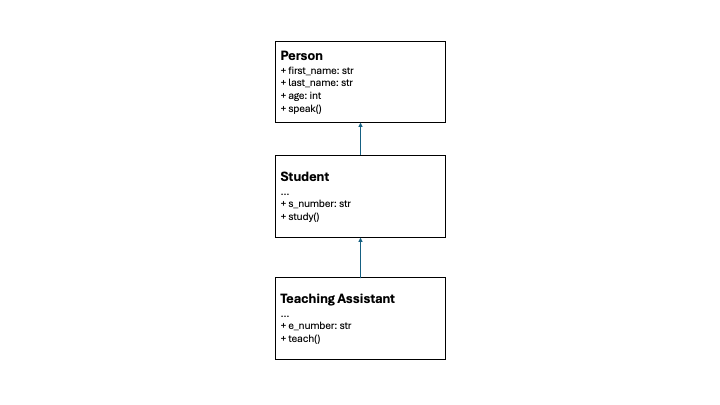
\includegraphics[scale=0.30]{images/hierarchy.png}
        \caption{our hierarchy}
        \label{fig:focuslogo}
    \end{figure}
\end{frame}

\begin{frame}[fragile]{Modifying the access}
\begin{minted}[fontsize=\footnotesize, breaklines]{python}
class Student(Person):
    def __init__(self, first_name, last_name, age, s_number):
        super().__init__(first_name, last_name, age)
        self.__s_number = s_number

# TeachingAssistant derives from Student
class TeachingAssistant(Student)
    def __init__(self, first_name, last_name, age, s_number, e_number):
            # Calling the constructor of Student
            super().__init__(first_name, last_name, age, s_number)
            self.__e_number = e_number

    def talk(self):
        print(f"Student {self.__s_number} is talking")
\end{minted}
\begin{itemize}
    \item Can we access it here?
\end{itemize}
\end{frame}

\begin{frame}[fragile]{Modifying the access again}
\begin{minted}[fontsize=\footnotesize, breaklines]{python}
class Student(Person):
    def __init__(self, first_name, last_name, age, s_number):
        super().__init__(first_name, last_name, age)
        self._s_number = s_number  # Removed one underscore

class TeachingAssistant(Student)
    def __init__(self, first_name, last_name, age, s_number, e_number):
            # Calling the constructor of Student
            super().__init__(first_name, last_name, age, s_number)
            self.__e_number = e_number

    def talk(self):
        print(f"Student {self._s_number} is talking")
\end{minted}
\begin{itemize}
    \item Is s\_number public, private or protected?
    \pause
    \item Can we access it in TeachingAssistant now?
\end{itemize}
\end{frame}

\begin{frame}[fragile]{Back to being private}
\begin{minted}[fontsize=\footnotesize, breaklines]{python}
class Student(Person):
    def __init__(self, first_name, last_name, age, s_number):
        super().__init__(first_name, last_name, age)
        self.__s_number = s_number  # It's private again!

class TeachingAssistant(Student)
    def __init__(self, first_name, last_name, age, s_number, e_number):
            # Calling the constructor of Student
            super().__init__(first_name, last_name, age, s_number)
            self.__e_number = e_number

    def change_student_number(self, new_student_number):
        self.__s_number = new_student_number
\end{minted}
\begin{itemize}
    \item Can we do this?
    \pause
    \item Not being able to access it, means we also shouldn't change it!
\end{itemize}
\end{frame}

\begin{frame}{Python being Python}
    \pause
    \begin{alertblock}{Access modifiers in Python (only for technical details)}
        In Python, access modifiers are not heavily enforced. Meaning, that if we wanted to, we can still access private/protected data attributes in places we shouldn't. However, it is the convention that you shouldn't! (And in the exam it is assumed they are heavily enforced).
    \end{alertblock}
    \begin{itemize}
        \item Other languages like Java, do heavily enforce their access modifiers.
    \end{itemize}
\end{frame}

\begin{frame}{Why are we doing this again?}
\begin{itemize}
    \item Why are we making our data attributes and methods private or protected?
    \pause
    \item \textbf{Encapsulation}
\end{itemize}
\end{frame}

    \section{Encapsulation}

\begin{frame}{The problem}
Why do we want to make our data attributes protected or private?
\begin{itemize}
    \pause
    \item Sometimes they contain information that shouldn't be known outside of the class
    \pause
    \item \textbf{We want to control how they are changed}
    \begin{itemize}
        \pause
        \item E.g., a student number should always start with a 's' and have 7 numbers.
        \pause
        \item A password should contain certain special characters
    \end{itemize}
    \pause
    \item Sometimes you want a data attribute to be able to be read, but not be able to be set. And the other way around.
\end{itemize}
\end{frame}

\begin{frame}{Solution to this problem}
\textbf{Solution:} we make methods that change our protected and private data attributes (\textbf{setters}) and/or make methods that return the value of our data attribute (\textbf{getters}).
\pause
\begin{itemize}
    \item We '\textbf{encapsulate}' our data attributes with \textit{getters} and/or \textit{setters}.
    \pause
    \item \textbf{This is encapsulation!}
\end{itemize}
\end{frame}

\begin{frame}[plain]
    Let's see how we do this in Python!
\end{frame}

\begin{frame}[fragile]{Making getters and setters}
\begin{minted}[fontsize=\footnotesize]{python}
class Student(Person):
    def __init__(self, first_name, last_name, age, s_number):
        super().__init__(first_name, last_name, age)
        self.__s_number = s_number  # Private data attribute
\end{minted}
\pause
\begin{minted}[fontsize=\footnotesize]{python}
    
    @property  # This is a decorator that indicates its a getter
\end{minted}
\pause
\begin{minted}[fontsize=\footnotesize]{python}
    def s_number(self):  # Note the name
\end{minted}
\pause
\begin{minted}[fontsize=\footnotesize]{python}
        return self.__s_number
\end{minted}
\pause
\begin{minted}[fontsize=\footnotesize]{python}

    @s_number.setter  # Decorator for setter
\end{minted}
\pause
\begin{minted}[fontsize=\footnotesize]{python}
    def s_number(self, new_s_number):  # Note the name
        if new_s_number.startswith("s"):
            self.__s_number = new_s_number
        else:
            raise ValueError
\end{minted}
\end{frame}

\begin{frame}[fragile]{Making getters and setters}
\begin{minted}[fontsize=\footnotesize]{python}
class Student(Person):
    ...
    @property  # This is a decorator that indicates its a getter
    def s_number(self):
        return self.__s_number

    @s_number.setter  # Decorator for setter
    def s_number(self, new_s_number):
        if new_s_number.startswith("s"):
            self.__s_number = new_s_number
        else:
            raise ValueError

student = Student("Daan", "Wichmann", "Secret", "s1234567")
# Because of the 'property' decorator we can use the getter
# as if s_number is just a normal data attribute
print(student.s_number)
>>> "s1234567"
\end{minted}
\end{frame}

\begin{frame}[fragile]{Making getters and setters}
\begin{minted}[fontsize=\footnotesize]{python}
class Student(Person):
    ...
    @property  # This is a decorator that indicates its a getter
    def s_number(self):
        return self.__s_number

    @s_number.setter  # Decorator for setter
    def s_number(self, new_s_number):
        if new_s_number.startswith("s"):
            self.__s_number = new_s_number
        else:
            raise ValueError

student = Student("Daan", "Wichmann", "Secret", "s1234567")
student.s_number = 1234567
print(student.s_number)
\end{minted}
What will happen?
\pause
\begin{minted}[fontsize=\footnotesize]{python}
>>> ValueError
\end{minted}
\end{frame}

\begin{frame}[fragile]{Making getters and setters}
\begin{minted}[fontsize=\footnotesize]{python}
class Student(Person):
    ...
    @property  # This is a decorator that indicates its a getter
    def s_number(self): 
        return self.__s_number

    @s_number.setter  # Decorator for setter
    def s_number(self, new_s_number):
        if new_s_number.startswith("s"):
            self.__s_number = new_s_number
        else:
            raise ValueError

student = Student("Daan", "Wichmann", "Secret", "s1234567")
student.s_number = s1020425
print(student.s_number)
\end{minted}
\pause
\begin{minted}[fontsize=\footnotesize]{python}
>>> "s1020425"
\end{minted}
\end{frame}

\begin{frame}{Encapsulation is important}
\begin{itemize}
    \item Encapsulation is one of the most important concepts of OOP!
    \pause
    \item Make sure to study it from the material, before the exam.
\end{itemize}
\pause
\begin{block}{Encapsulation (definition from the material)}
    Hiding attributes from clients is called encapsulation. As the name implies, the attribute is "enclosed in a capsule". The client is then offered a suitable interface for accessing and processing the data stored in the object.
\end{block}
\pause
\begin{itemize}
    \item Client := your program
    \item The suitable interface that is referred to are the getters and setters
\end{itemize}
\end{frame}

    \section{Seperation of Concerns}

\begin{frame}{Separation of Concerns}
\begin{block}{Separation of Concerns}
Separation of concerns is a design principle for separating a computer program into distinct sections such that each section addresses a separate concern. A concern is a set of information that affects the code of a computer program.
\end{block}
\end{frame}

\begin{frame}{Separation of Concerns}
\begin{itemize}
    \item One of the most important concepts of OOP! (together with encapsulation).
    \item Classes separate our program into different parts
    \item This makes it so that one part of the program does not have to be \textbf{concerned} with another part of our program.
    \item \textbf{Encapsulation} facilitates this by hiding the implementation of our classes behind well defined interfaces (e.g. getters and setters).
    \begin{itemize}
        \pause
        \item So other classes don't have to be concerned with how a variable is changed or read.
    \end{itemize}
    \item \textbf{In a nutshell:} a class should only do what it is designed to do.
\end{itemize}
\end{frame}

\begin{frame}{Why you should use OOP!}
Why you should know about seperation of concerns and encapsulation.
\end{frame}

\begin{frame}{Why you should use OOP!}
Let's say you have a group project, to create a phone book app.
\begin{itemize}
    \pause
    \item You create a \textbf{PhoneBook} class that stores phone numbers.
    \pause
    \item You want to be able to add and see phone numbers via the terminal.
    \pause
    \item (Following seperation of concerns) you create a different class \textbf{PhoneBookApplication} that handles the input, output, and the loop of your program.
    \pause
    \item You also want to maintain a database with all phone numbers (e.g. txt file, CSV file, or MySQL database).
    \pause
    \item So, you create another class that interacts with a database \textbf{DatabaseHandler}
\end{itemize}
\end{frame}

\begin{frame}{Why you should use OOP!}
\begin{itemize}
    \item Let's assume person A made the PhoneBook class, person B made the PhoneBookApplication class, and person C made the DatabaseHandler class.
    \pause
    \item By creating different classes you can divide the work nicely!
    \pause
    \item Lets assume all classes have well defined methods.
    \pause
    \item For example, the DatabaseHandler has a method save\_to\_database(phonebook).
    \pause
    \item Only person C has to be concerned with how this method works, and has to make sure that it saves to a database.
    \pause
    \item Person B needs to use this method, but does not need to be \textbf{concerned} with how it works! The implementation is \textbf{encapsulated} behind the method.
\end{itemize}
\end{frame}

\begin{frame}{Why you should use OOP!}
    \begin{itemize}
        \item Separation of Concerns and encapsulation makes creating big projects (in groups) way easier!
    \end{itemize}
\end{frame}

    \section{Class attributes}

\begin{frame}{What are class attributes?}
\pause
\begin{block}{Class attributes (definition)}
    Class attributes are \textbf{data attributes} or \textbf{methods}, that do not belong to instances of a class, but to the class itself.
\end{block}
\pause
\begin{itemize}
    \item Class data attributes
    \pause
    \item Class methods
\end{itemize}
\end{frame}

\begin{frame}[fragile]{An example...}
\pause
\begin{minted}{python}
class Person():
    ...

    # An oridinary method :o
    def greet(self):
        print("Hey!")
\end{minted}
\end{frame}

\begin{frame}[fragile]{Hmmmmm...}
\pause
\begin{minted}{python}
person1 = Person("Daan", "Wichmann", 19)
\end{minted}
\pause
\begin{minted}{python}
person2 = Person("Ella", "Kemperman", 19)
\end{minted}
\pause
\begin{minted}{python}
person1.greet()
>>> "Hey!"
\end{minted}
\pause
\begin{minted}{python}
person2.greet()
>>> "Hey!"
\end{minted}
\pause
\begin{itemize}
    \item Different objects, same output!
    \pause
    \item We can do this better!
\end{itemize}
\end{frame}

\begin{frame}[fragile]{Wow it's a classmethod!}
\pause
\begin{minted}{python}
class Person():
    ...

    @classmethod # Only the decorator is added!
    def greet(cls):  # Note the first parameter!
        print("Hey!")
\end{minted}
\end{frame}

\begin{frame}[fragile]{Same for data attributes!}
\pause
\begin{itemize}
    \item If the values are the same for every object, we can make it a class data attribute!
\end{itemize}
\begin{minted}{python}
class Person():
    greeting = "Hey! # Class data attribute

    @classmethod
    def greet(cls):
        print(cls.greeting)
\end{minted}
\end{frame}
    
    \begin{frame}[focus]
        That is it!
        
        (make sure to still look at the material!)
    \end{frame}

    \begin{frame}{NB}
        I did not cover \textbf{class attributes}. Please study this in your own time, because it is still fairly important! (Part 9.5 of the material)
    \end{frame}
    
    \begin{frame}{Extra info}
        \usebeamercolor[fg]{normal text}
        If you are interested in programming, I highly recommend following: Object Orientend Programming (NWI-IPI005)
        \vfill
        You can find these slides and the code from the presentation on my github: \texttt{https://github.com/D21W12}
    \end{frame}
\end{document}
